\documentclass{article}
% Margin definition.
\usepackage[a4paper,total={6.8in, 8.5in}]{geometry}
\usepackage{parskip}
% Images.
\usepackage{graphicx}
\usepackage[hidelinks, bookmarks=true]{hyperref}
\usepackage{float}
% Encoding.
\usepackage[english]{babel}
\usepackage[utf8]{inputenc}
% Helvetic font.
\usepackage[scaled]{helvet}
\renewcommand\familydefault{\sfdefault} 
% Header for UA logo.
\usepackage{fancyhdr}
% Dots in index.
\usepackage[titles]{tocloft}
\renewcommand{\cftsubsecleader}{\Large\cftdotfill{0}}
\renewcommand{\cftsecleader}{\Large\cftdotfill{0}}
\renewcommand{\cftsecfont}{\large\bfseries\scshape}
\renewcommand{\cftsubsecfont}{\scshape}
\renewcommand*{\HyperDestNameFilter}[1]{\jobname-#1}
% Dot after number in (sub)sections and in toc.
\renewcommand{\cftsecaftersnum}{.}
\renewcommand{\cftsubsecaftersnum}{.}
\usepackage{titlesec}
\titlelabel{\hspace{-0.5cm}\quad}
\usepackage[letterspace=45]{microtype}
\newcommand*{\fullref}[1]{\hyperref[{#1}]{\autoref*{#1} \nameref*{#1}}}
% Header with UA logo definition. 
\pagestyle{fancy}
\fancyhf{}
\chead{
    
\includegraphics[width=5in]{./images/header_ua.png}
}
\setlength\headheight{20pt}
% Footer with page number.
\rfoot{Page \thepage}
\renewcommand{\footrulewidth}{0.1pt}
% Rename table of contents title to "Index"
\renewcommand{\contentsname}{\normalsize Index \vspace{0.6cm}}
% Water mark
\newsavebox\mybox
\usepackage[printwatermark]{xwatermark}
\usepackage{xcolor}
\usepackage{tikz}
% paragraph
\newcommand\tab[1][1cm]{\hspace*{#1}}
\setlength\parindent{24pt}
%images
 \usepackage{graphicx}
\usepackage{caption}
% footnotes at bottom
\usepackage[bottom]{footmisc}
% Urls with line break
\usepackage{pdflscape}
% Drawing functions
\usepackage{tikz}
\usepackage{pgfplots}
\pgfplotsset{width=7cm, height=4cm, compat=1.17}

\usepackage{multicol}
\setlength{\columnsep}{1cm}

%%%%%%%%%%%% References/Bibliography %%%%%%%%%%%%
\usepackage{biblatex}
\addbibresource{bibliography.bib}

%%%%%%%%%%%%%%%%%%%%%%%%%%%%%%%%%%%%%%%%%%%%%%%%%

\begin{document}

%%%%%%%%%%%%%%%%%% Cover Page %%%%%%%%%%%%%%%%%%
\title{\vspace{-0.9cm}
       \vspace{1cm}
       \normalsize
       \raggedright\textbf{Title: \hspace{1.5cm} Anatomy of a Web Connection: A Brief Analysis} \\ \vspace{0.4cm}
       \raggedright\textbf{Autor: \hspace{1.3cm} Eduardo Santos} \\ \vspace{0.4cm}
       \raggedright\textbf{Date: \hspace{1.45cm} 21/03/2021} \\}
\author{}
\date{}

\maketitle
\thispagestyle{fancy}

%%%%%%%%%%%%%%%%%% END Cover Page %%%%%%%%%%%%%%%%%%

\vspace{-1.4cm}

\tableofcontents


\fontsize{10pt}{13pt}
\selectfont
\lsstyle

\titlelabel{\thetitle.\quad}	

\section{Introductory Note}

\tab This assignment consists in the use of the \textit{traceroute} command followed by the domain "www.cmu.edu", and interpreting the results obtained.  

\noindent The specific objectives of this assignment are the following:

\begin{itemize}
    \item To provide a plausible identification of the technologies, processes, actors and business models involved in an web connection.
    \item To identify possible social and economic implications associated with the identified technologies, processes, actors and business models.
\end{itemize}

\section{Summary / Abstract}

\tab This assignment addresses things that can happen during a web connection.

Using the \textit{traceroute} command, we will be able to analyze how a web connection works, and the path that the packages take in that connection.
From that analysis, we will be able to reach a conclusion about the previously referred paths, and the hops of the connection, referring also the players involved in each hop.

This assignment will also contemplate some other points, such as the operations, processes, techniques and technologies involved in each step, trying to situate these in the framework of the ISO OSI model, as well as some possible social and economic implications triggered by the point previously mentioned.

\section{Framework}

The web as a major importance in our lives, without it, most of our daily common tasks, tasks that we consider easy, wouldn't be so easy as we wished to. 

We can find an entire "world" inside our computers, smartphones, etc. This is only possible because there are many technologies, processes and actors involved, all of them through an abstract layer that hides the real complexity of the whole system. The operations inside that layer might have significant social and economic implications.

\section{Protocols and mechanisms involved in a web connection}

\tab In an Internet connection, there are 2 main participants: clients and servers.

Clients are devices that are connected to the Internet, they can be computers, smartphones, etc. Servers are also devices (specifically computers), they can store webpages, sites or apps. 
When a client makes a request to access a specific webpage, the server responds with a copy of the webpage, which is downloaded to the client's machine. This copy is then displayed in the user's web browser.

This is how a web connection works, at least at a very high-level. But there are many other parts involved in the connection. We will see a brief explanation of some of the mechanisms used during this connection.

\subsection{Web browser}

\tab A web browser is a software application that is used for accessing the WWW\footnote{World Wide Web}. When a user makes a request for a web page, the web browser responds with the content from a web server, displaying the same content on the user's device/machine. That content is transferred using the Hypertext Transfer Protocol, which defines how text, images and videos are transmitted through machines on the web. We will address this protocol later on.

Websites save information about its users in files, those files are called cookies. They are stored in our computers for the next time we visit that website. For example, when we choose the option to store our username/email and password, that is made possible with the usage of cookies.

A web browser should not be confused with a search engine, the last one being a website that contains links to other websites.

\subsection{TCP/IP}

\tab TCP\footnote{Transmission Control Protocol} and IP\footnote{Internet Protocol} are often referred together as TCP/IP, an Internet protocol suite. This suite is a set of communications protocols, establishing how data should be packetized, addressed, transmitted, routed, and received in an end-to-end data communication.

Architecturally speaking, TCP/IP can be divided into a four-layer model, which consists in the following layers:

\begin{itemize}
    \item \textbf{Application layer} - scope within which applications, or processes, create user data and communicate this data to other applications, this can be done on the same host, or on a different one;
    \item \textbf{Transport layer} - performs host-to-host communications, this communications can be on the local network, as well as on remote networks (separated by routers);
    \item \textbf{Internet layer} - provides a uniform networking interface that hides the actual topology of the underlying network connections;
    \item \textbf{Link layer} - defines the networking methods within the scope of the local network link on which hosts communicate, this is done without routers.
\end{itemize}

\subsection{DNS} 

\tab DNS\footnote{Domain Name System} is a naming system for computers, services, or other resources connected to the Internet, although it can also be done in a private network.

The way that humans access information online is through domain names, unlike web browsers, that interact through IP addresses. DNS job is to translate these domain names to IP addresses.

We've seen that web browsers communicate through IP addresses, but what is an IP address?

An IP address is an unique address that identifies a device on the Internet or a local network. Using this address, machines can find each other on that network.

\subsection{HTTP}

\tab HTTP\footnote{Hypertext Transfer Protocol} is an application-layer protocol used when transmitting hypermedia documents (such as HTML\footnote{Hypertext Markup Language}). It was designed for communications between web browsers and web servers, although it can be used for other purposes. 

This protocol follows a client-server model, a client opens a connection and makes a request, then waits to receive the response. Being a stateless protocol, the server doesn't store any data between two requests.

\section{Traceroute command}

\tab Traceroute is a network diagnostic tool used for real-time tracking of the path taken by a packet on an IP network, from source to destination. This tool also reports the IP addresses of all the routers it pinged in between, recording also the time taken for each hop the packet makes during its route.

Traceroute normally uses ICMP\footnote{Internet Control Message Protocol} echo packets with variable TTL\footnote{Time To Live}. For accuracy aspects, each hop is queried usually three times to better measure the response. 

However, Traceroute messages are often blocked in the Internet by routers, making this tool very inaccurate in some cases.

\section{Executing the \textit{traceroute} command}

\tab Executing the command \textit{traceroute -I www.cmu.edu}, we obtain the following output:

%Added [H] after so that image is placed after the text above
%This is only possible by adding also \usepackage{float} to the preamble
\begin{figure}[H]
    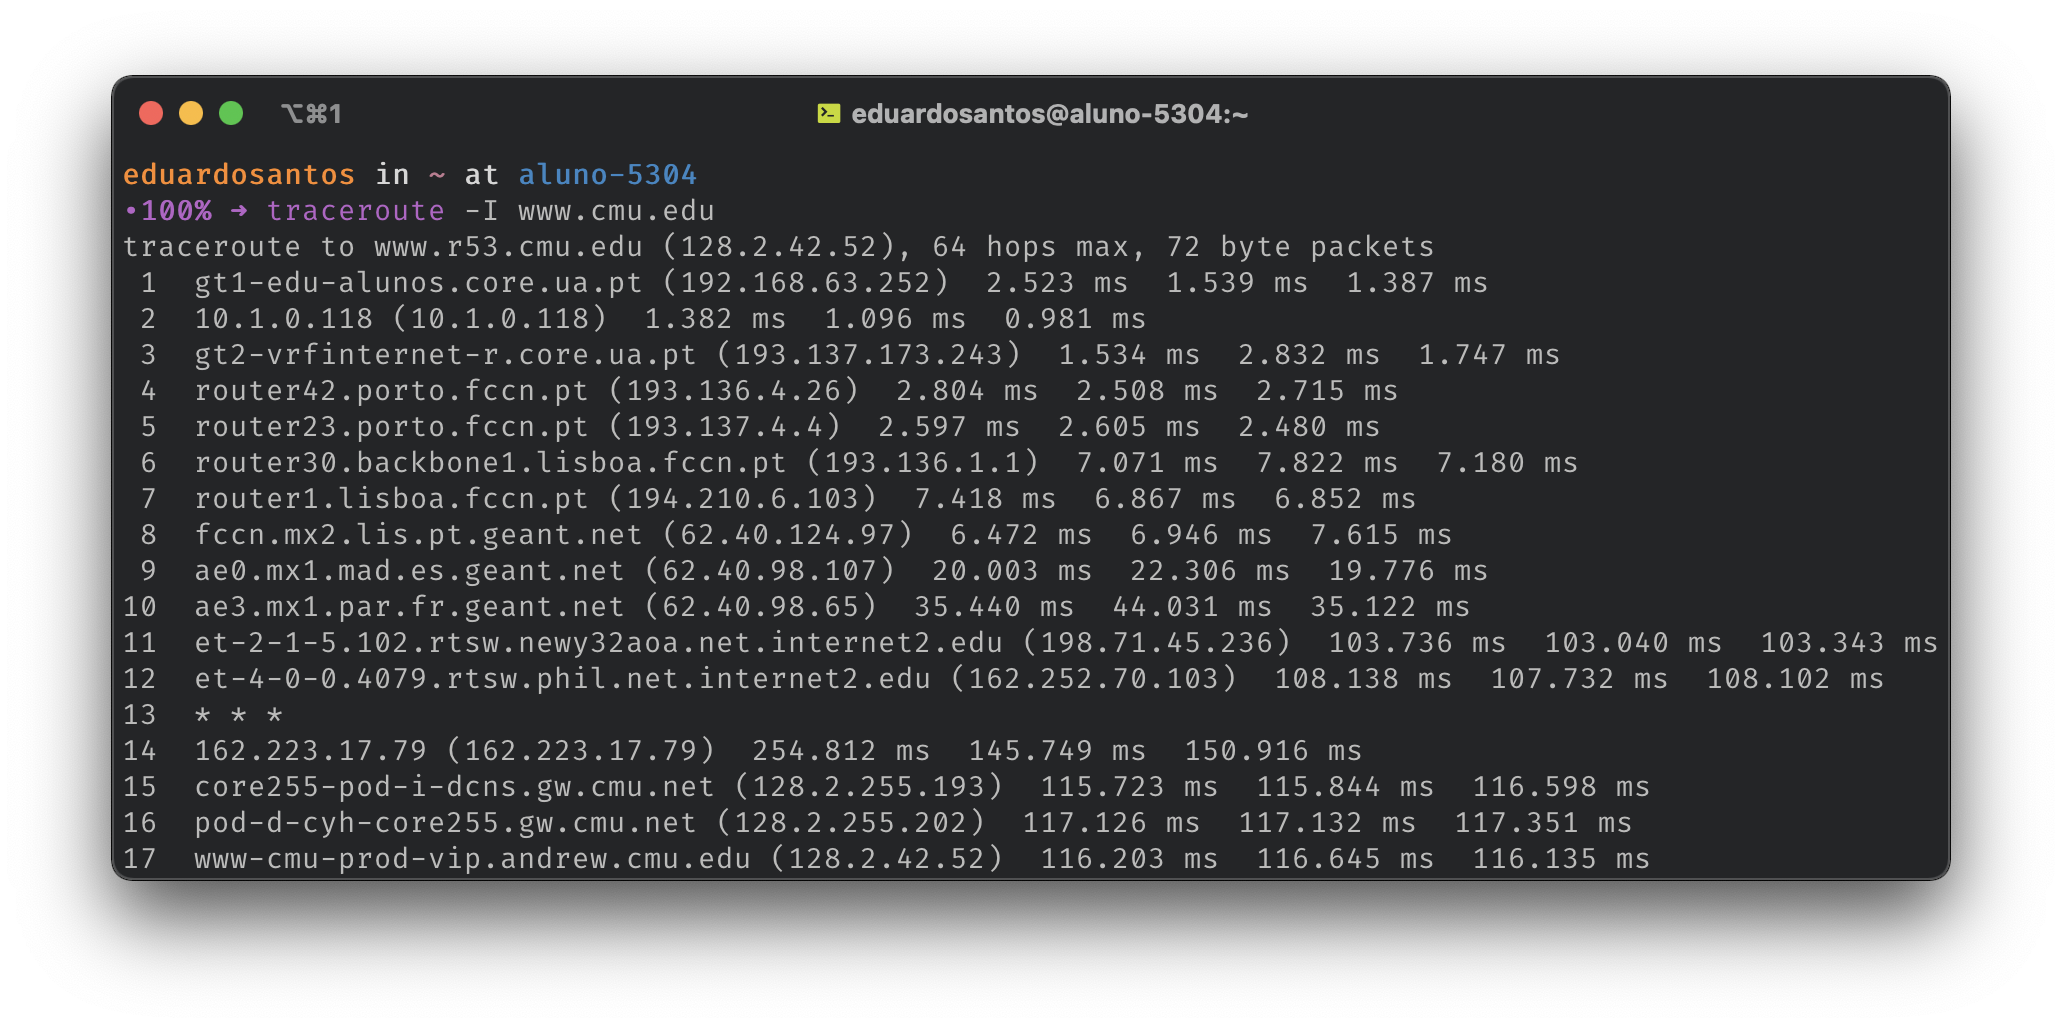
\includegraphics[width=1 \textwidth]{images/tracerouteUA.png}
    \caption{Output of the \textit{traceroute} command}
\end{figure}

\subsection{Detailed interpretation of the executed command's results}

\vspace*{\fill}
\begin{center}
    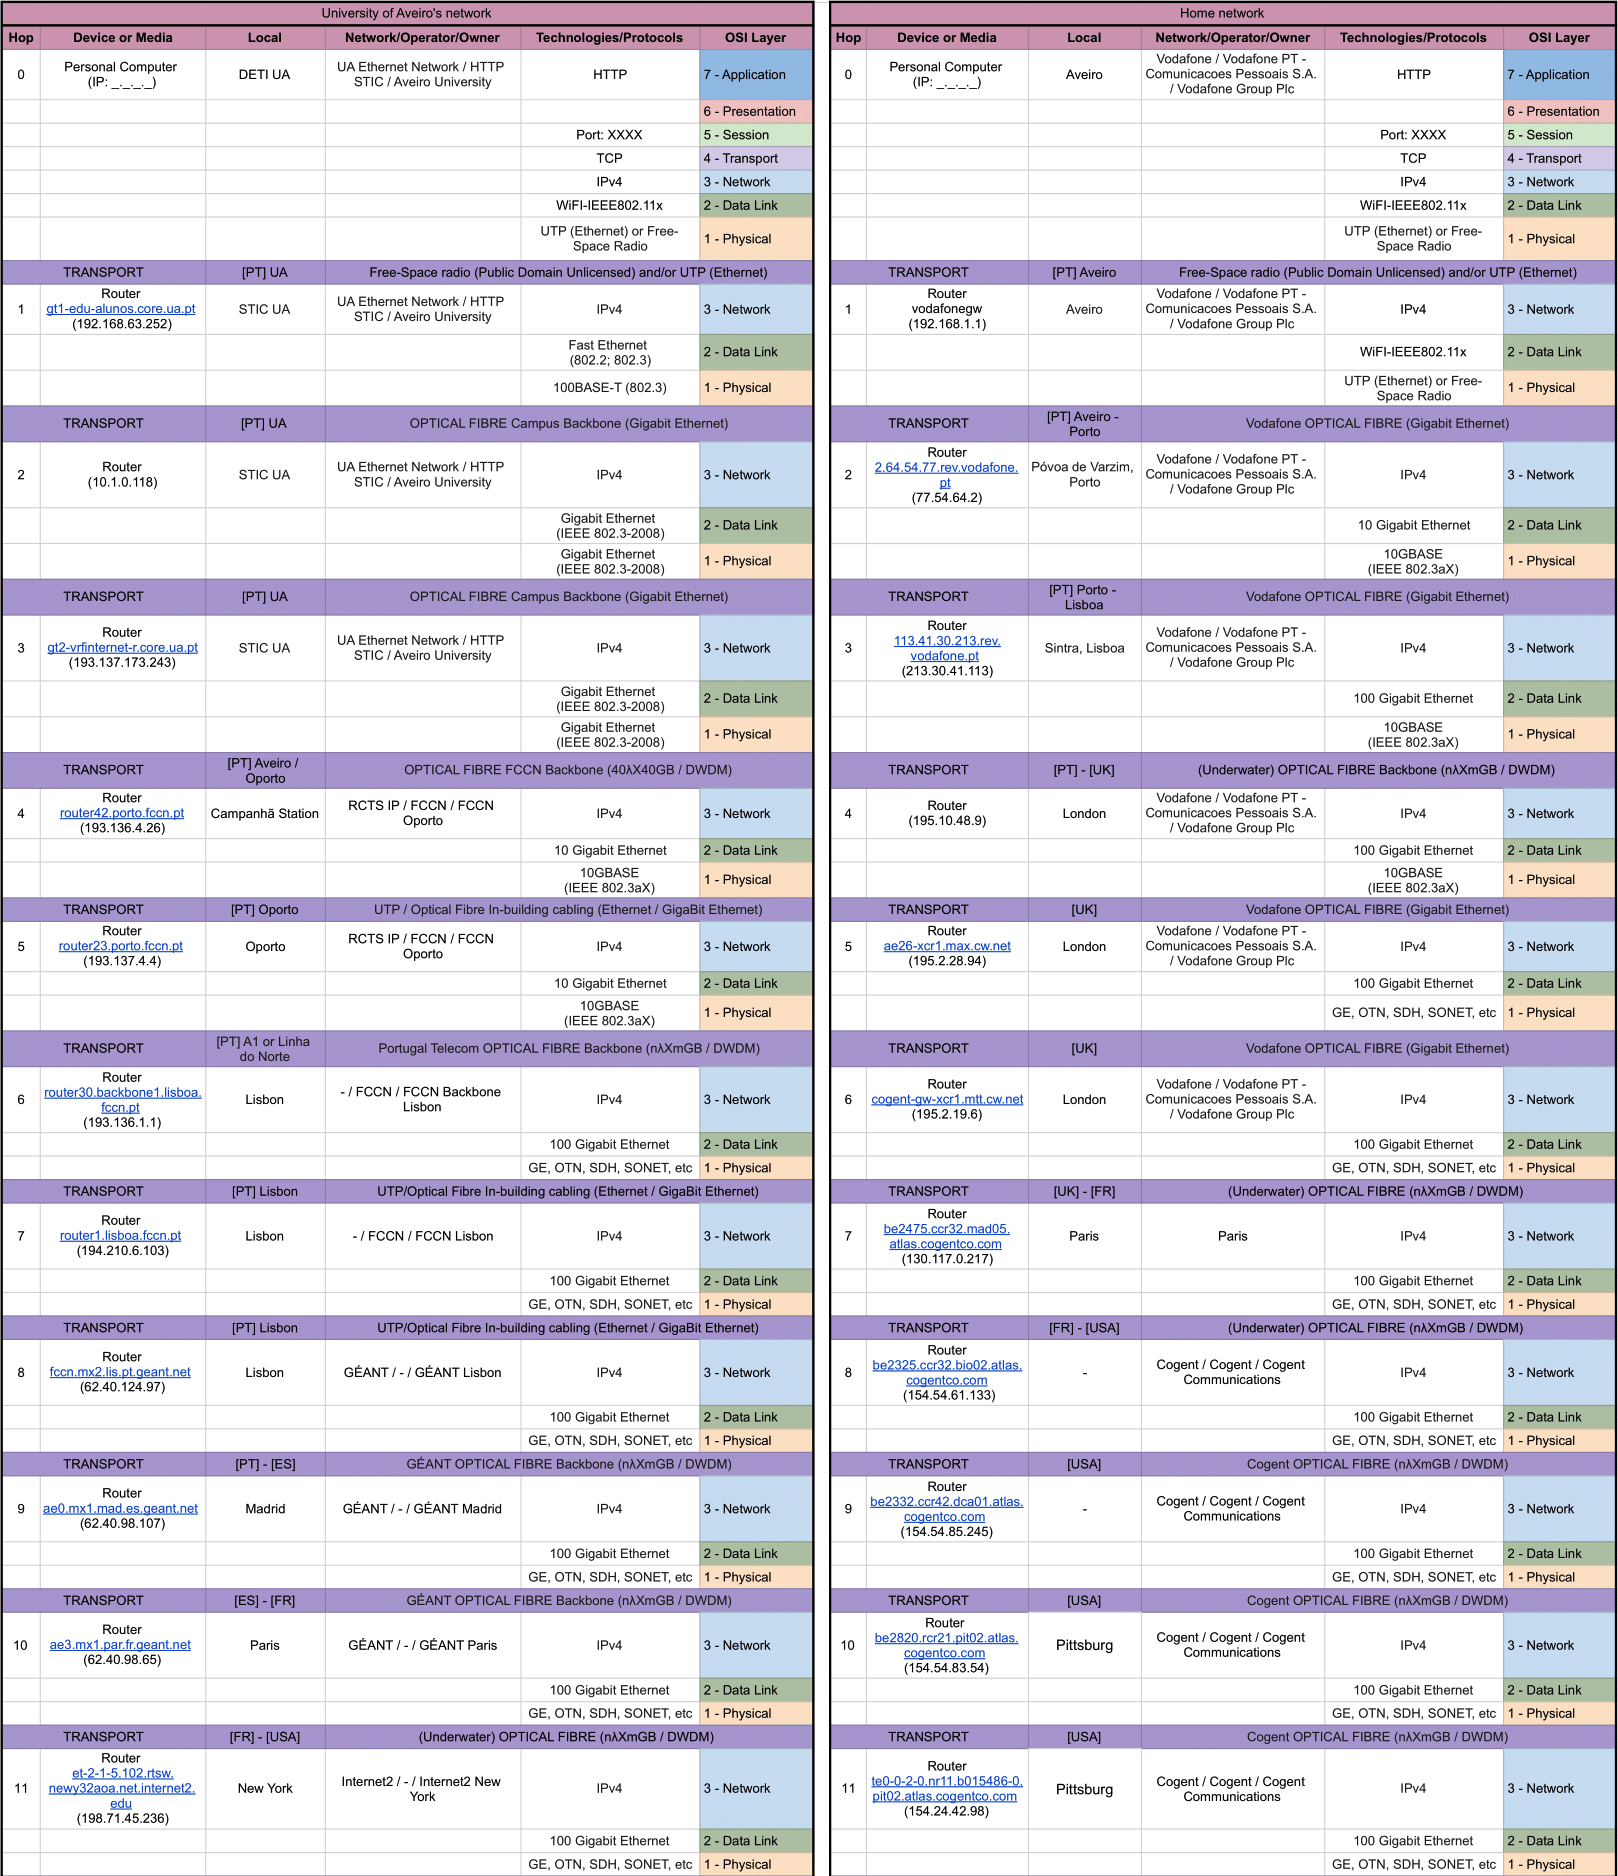
\includegraphics[width=1 \textwidth]{images/traceroute_part1.png}
\end{center}
\vspace*{\fill}\clearpage

\vspace*{\fill}
\begin{center}
    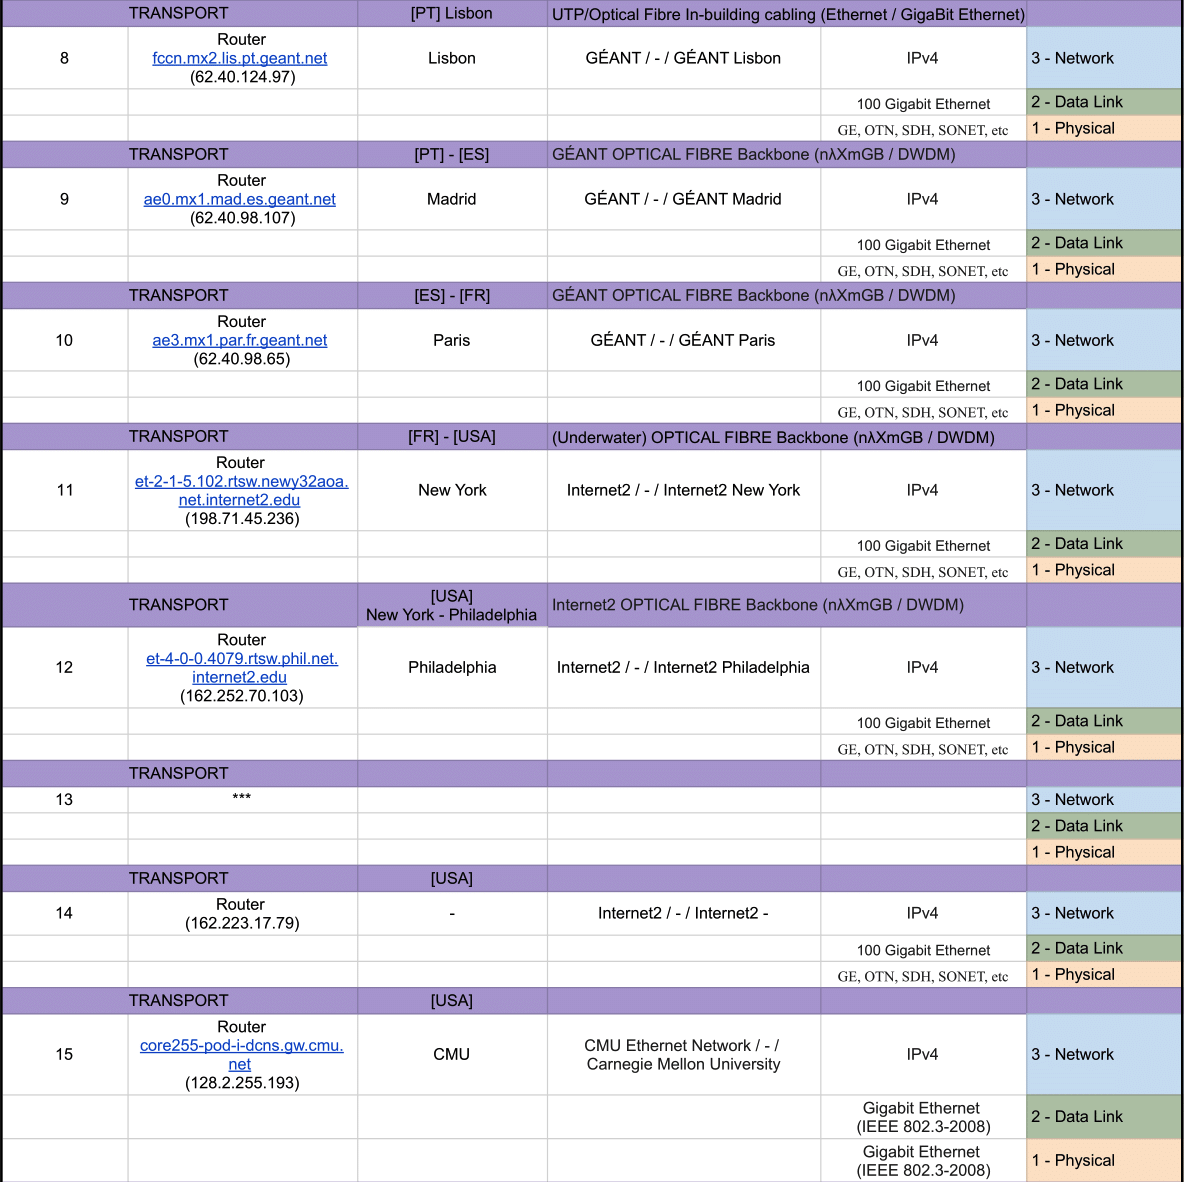
\includegraphics[width=1 \textwidth]{images/traceroute_part2.png}
\end{center}
\vspace*{\fill}\clearpage

\begin{figure}
    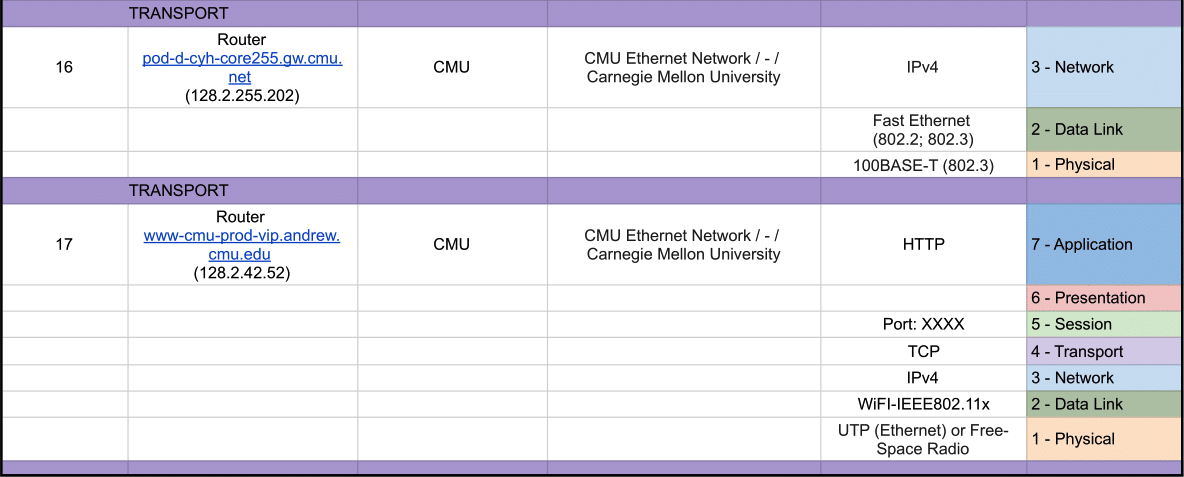
\includegraphics[width=1 \textwidth]{images/traceroute_part3.png}
    \caption{Details of \textit{traceroute} interpretation}
\end{figure}

% Add "References" to table of contents
\addcontentsline{toc}{section}{References}
% No cite makes all references appear, even if there's no citation on the text
\nocite{*}
\printbibliography

\end{document}